\documentclass[11pt,a4paper]{article}
\usepackage[T1]{fontenc}
\usepackage[utf8]{inputenc}
\usepackage[provide=*,italian]{babel}
\usepackage{lmodern,microtype}
\usepackage{geometry}
\geometry{margin=2.5cm}
\usepackage{amsmath,amssymb,amsthm,mathtools}
\usepackage{booktabs,array,longtable}
\usepackage{xcolor,enumitem}
\usepackage{tikz}
\usetikzlibrary{arrows.meta,positioning,calc}
\usepackage[most]{tcolorbox}
\usepackage{listings}
\usepackage{hyperref,fancyhdr}

\definecolor{sapienzared}{RGB}{130,0,36}
\definecolor{softred}{RGB}{249,241,243}
\definecolor{softblue}{RGB}{239,246,252}
\definecolor{softgray}{RGB}{245,245,245}
\definecolor{codegreen}{RGB}{25,110,65}
\hypersetup{colorlinks=true,linkcolor=sapienzared,urlcolor=sapienzared,
pdftitle={Alberi e grafi aciclici},pdfauthor={Giampaolo Liuzzi}}

\pagestyle{fancy}
\fancyhf{}
\fancyhead[L]{\small Ottimizzazione su Reti}
\fancyhead[R]{\small Capitolo 3}
\fancyfoot[C]{\thepage}
\renewcommand{\headrulewidth}{0.4pt}

\newtheorem{definition}{Definizione}[section]
\newtheorem{theorem}[definition]{Teorema}
\newtheorem{proposition}[definition]{Proposizione}
\newtheorem{observation}[definition]{Osservazione}

\newtcolorbox{learningbox}{colback=softred,colframe=sapienzared,
title=Obiettivi di apprendimento,fonttitle=\bfseries,boxrule=0.8pt,arc=1.5mm}
\newtcolorbox{examplebox}[1]{colback=softblue,colframe=blue!55!black,
title=#1,fonttitle=\bfseries,boxrule=0.7pt,arc=1.5mm}
\newtcolorbox{notationbox}{colback=softgray,colframe=black!55,
title=Registro delle notazioni,fonttitle=\bfseries,boxrule=0.7pt,arc=1.5mm}
\newtcolorbox{warningbox}{colback=yellow!9,colframe=orange!65!black,
title=Attenzione,fonttitle=\bfseries,boxrule=0.7pt,arc=1.5mm}
\newtcolorbox{networkxbox}{colback=softgray,colframe=black!55,
title=Python/NetworkX,fonttitle=\bfseries,boxrule=0.7pt,arc=1.5mm}

\lstdefinestyle{python}{language=Python,basicstyle=\ttfamily\small,
keywordstyle=\color{blue!65!black}\bfseries,commentstyle=\color{codegreen},
stringstyle=\color{sapienzared},backgroundcolor=\color{softgray},frame=single,
rulecolor=\color{black!25},showstringspaces=false,breaklines=true,columns=fullflexible}

\newcommand{\V}{\mathcal{V}}
\newcommand{\E}{\mathcal{E}}
\newcommand{\R}{\mathbb{R}}
\newcommand{\deltaout}{\delta^{+}}
\newcommand{\deltain}{\delta^{-}}

\begin{document}
\hypersetup{pageanchor=false}
\begin{titlepage}
\centering
\vspace*{1.6cm}
{\color{sapienzared}\rule{\textwidth}{1.2pt}}\\[1.1cm]
{\Large Ottimizzazione su Reti}\\[0.35cm]
{\huge\bfseries Capitolo 3}\\[0.45cm]
{\LARGE\bfseries Alberi e grafi aciclici}\\[1.1cm]
{\color{sapienzared}\rule{0.72\textwidth}{0.8pt}}\\[1.1cm]
{\large Corso di Laurea Magistrale in Ingegneria Gestionale}\\[0.25cm]
{\large Sapienza Università di Roma}\\[1.2cm]
{\large Giampaolo Liuzzi}\\[0.25cm]
{\normalsize Dipartimento di Ingegneria Informatica, Automatica e Gestionale}\\[2cm]
\vfill
{\small Versione preliminare per uso didattico}
\end{titlepage}
\hypersetup{pageanchor=true}
\pagenumbering{roman}
\tableofcontents
\newpage
\pagenumbering{arabic}

\begin{learningbox}
Al termine del capitolo lo studente dovrebbe essere in grado di:
\begin{itemize}[nosep]
\item riconoscere alberi e foreste e usarne le caratterizzazioni equivalenti;
\item costruire e verificare un albero ricoprente;
\item comprendere il ruolo di un albero nella matrice di incidenza;
\item distinguere alberi non orientati e arborescenze;
\item riconoscere un grafo orientato aciclico e calcolarne un ordinamento topologico;
\item implementare le operazioni fondamentali mediante NetworkX.
\end{itemize}
\end{learningbox}

\section{Grafi aciclici, foreste e alberi}

In questa prima parte $G=(\V,\E)$ è un grafo \emph{non orientato}, finito e semplice.

\begin{definition}[Foresta e albero]
Un grafo che non contiene cicli è detto \emph{aciclico} o \emph{foresta}. Un grafo aciclico e connesso è detto \emph{albero}.
\end{definition}

Le componenti connesse di una foresta sono alberi. Un singolo nodo, privo di spigoli, è dunque un albero. Questa convenzione evita eccezioni nelle proprietà ricorsive.

\begin{definition}[Foglia]
In un albero $T=(\V,\E)$ con almeno due nodi, un nodo $v$ di grado $d(v)=1$ è detto \emph{foglia}. Il suo unico vicino è talvolta detto padre quando si sceglie una radice.
\end{definition}

\begin{proposition}
Ogni albero con almeno due nodi possiede almeno due foglie.
\end{proposition}

\emph{Idea della dimostrazione.} Si consideri un cammino semplice di lunghezza massima. Se uno dei suoi estremi avesse un vicino non appartenente al cammino, lo si potrebbe prolungare; se avesse un altro vicino sul cammino, si formerebbe un ciclo. Entrambi gli estremi hanno quindi grado uno.

\section{Caratterizzazioni equivalenti degli alberi}

\begin{theorem}[Proprietà fondamentali]
Per un grafo $G=(\V,\E)$ con $n=|\V|$, le seguenti affermazioni sono equivalenti:
\begin{enumerate}[label=\arabic*.]
\item $G$ è un albero;
\item ogni coppia di nodi è collegata da un unico cammino;
\item $G$ è aciclico e $|\E|=n-1$;
\item $G$ è connesso e $|\E|=n-1$;
\item $G$ è aciclico e l'aggiunta di uno spigolo tra due nodi non adiacenti crea un unico ciclo;
\item $G$ è connesso e l'eliminazione di un qualsiasi spigolo lo rende non connesso.
\end{enumerate}
\end{theorem}

Queste equivalenze esprimono due modi complementari di vedere un albero: è \emph{massimalmente aciclico} e, nello stesso tempo, \emph{minimamente connesso}.

\begin{examplebox}{Un controllo rapido}
Un grafo con $8$ nodi, $7$ spigoli e connesso è necessariamente un albero. La sola uguaglianza $|\E|=|\V|-1$, invece, non basta: un grafo può contenere un ciclo in una componente e avere un'altra componente isolata.
\end{examplebox}

\subsection{Conteggio degli spigoli in una foresta}

\begin{proposition}
Se una foresta ha $n$ nodi e $k$ componenti connesse, allora
\[
|\E|=n-k.
\]
In particolare, per un albero $k=1$ e $|\E|=n-1$.
\end{proposition}

\section{Alberi ricoprenti}

\begin{definition}[Albero ricoprente]
Dato un grafo connesso $G=(\V,\E)$, un sottografo $T=(\V,F)$ è un \emph{albero ricoprente} di $G$ se $F\subseteq\E$ e $T$ è un albero.
\end{definition}

L'aggettivo ``ricoprente'' indica che $T$ contiene tutti i nodi di $G$, ma soltanto $n-1$ dei suoi spigoli. Un grafo possiede un albero ricoprente se e solo se è connesso.

\begin{figure}[ht]
\centering
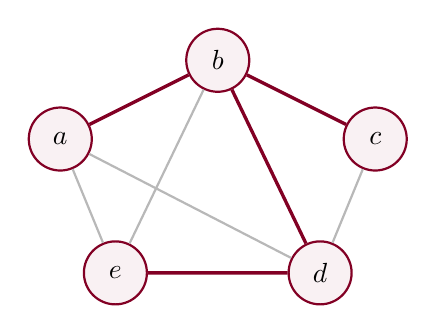
\begin{tikzpicture}[node/.style={circle,draw=sapienzared,thick,fill=softred,minimum size=8mm},
all/.style={black!28,thick},tree/.style={sapienzared,very thick}]
\foreach \x/\y/\z in {a/0/1.7,b/2/2.7,c/4/1.7,d/3.3/0,e/0.7/0}
  \node[node] (\x) at (\y,\z) {$\x$};
\draw[all] (a)--(b)--(c)--(d)--(e)--(a);
\draw[all] (a)--(d) (b)--(d) (b)--(e);
\draw[tree] (a)--(b)--(c);
\draw[tree] (b)--(d)--(e);
\end{tikzpicture}
\caption{In rosso un albero ricoprente: collega tutti i cinque nodi con quattro spigoli.}
\end{figure}

\subsection{Costruzione incrementale}

Un albero ricoprente può essere costruito sfruttando i tagli introdotti nel Capitolo 2.

\begin{enumerate}
\item Scegliere $r\in\V$ e porre $S=\{r\}$, $F=\varnothing$.
\item Finché $S\neq\V$, scegliere uno spigolo $e=\{u,v\}\in\delta(S)$ con $u\in S$ e $v\notin S$.
\item Porre $S\leftarrow S\cup\{v\}$ e $F\leftarrow F\cup\{e\}$.
\end{enumerate}

Se a un certo passo $\delta(S)=\varnothing$, il grafo non è connesso. Altrimenti, ogni iterazione aggiunge un nodo e uno spigolo senza creare cicli; al termine $T=(\V,F)$ è un albero ricoprente.

\begin{warningbox}
L'algoritmo non specifica quale spigolo del taglio scegliere. Scelte diverse possono produrre alberi ricoprenti diversi. Se agli spigoli sono associati costi e si sceglie sempre uno spigolo di costo minimo ammissibile, si entra nel problema dell'albero ricoprente di costo minimo.
\end{warningbox}

\section{Scambio di spigoli e ciclo fondamentale}

Sia $T=(\V,F)$ un albero ricoprente di $G$ e sia $e=\{u,v\}\in\E\setminus F$. In $T$ esiste un unico cammino tra $u$ e $v$; aggiungendo $e$ si crea quindi un unico ciclo, detto \emph{ciclo fondamentale} di $e$ rispetto a $T$.

Se dal ciclo fondamentale si elimina uno spigolo $f\neq e$, si ottiene
\[
F'=F\cup\{e\}\setminus\{f\},
\]
e $(\V,F')$ è ancora un albero ricoprente. Questa operazione di scambio sarà essenziale nel simplesso su reti: un arco entra nella base, si crea un ciclo e un altro arco esce.

\section{Alberi e matrice di incidenza}

Sia $G=(\V,\E)$ un grafo orientato ottenuto assegnando un verso arbitrario agli spigoli di un grafo connesso. Manteniamo la convenzione fissata:
\[
A_{ie}=\begin{cases}
-1,&\text{se il nodo $i$ è l'origine dell'arco $e$},\\
+1,&\text{se il nodo $i$ è la destinazione dell'arco $e$},\\
0,&\text{altrimenti.}
\end{cases}
\]

\begin{theorem}[Rango della matrice di incidenza]
Se $G$ è connesso e $|\V|=n$, allora $\operatorname{rank}(A)=n-1$. Eliminando una riga qualsiasi di $A$ si ottiene la matrice ridotta $\bar A$; un insieme $F$ di $n-1$ colonne di $\bar A$ è linearmente indipendente se e solo se gli archi di $F$, considerati senza orientamento, formano un albero ricoprente.
\end{theorem}

L'orientamento scelto modifica soltanto il segno di alcune colonne e non l'indipendenza lineare. Il teorema stabilisce il ponte tra la struttura combinatoria degli alberi e le basi algebriche impiegate nel Capitolo 4.

\begin{examplebox}{Matrice ridotta di un albero}
Per gli archi $(1,2)$, $(1,3)$ e $(3,4)$, eliminando la riga del nodo $1$ si ottiene
\[
\bar A=
\begin{pmatrix}
1&0&0\\
0&1&-1\\
0&0&1
\end{pmatrix},
\qquad \det(\bar A)=1.
\]
Le tre colonne corrispondono a un albero sui quattro nodi e formano una base.
\end{examplebox}

\section{Alberi radicati e arborescenze}

Un albero non orientato diventa \emph{radicato} quando si distingue un nodo $r$, detto radice. La distanza dalla radice definisce i livelli; ogni nodo diverso da $r$ ha un unico padre e può avere zero o più figli.

\begin{definition}[Arborescenza uscente]
Un digrafo $T=(\V,F)$ è un'\emph{arborescenza uscente} radicata in $r$ se, per ogni $v\in\V\setminus\{r\}$, esiste un unico cammino orientato da $r$ a $v$.
\end{definition}

In un'arborescenza uscente, $d^-(r)=0$ e $d^-(v)=1$ per ogni $v\neq r$. In modo simmetrico, in un'\emph{arborescenza entrante} esiste un unico cammino orientato da ogni nodo verso $r$; quindi $d^+(r)=0$ e $d^+(v)=1$ per $v\neq r$.

\begin{warningbox}
Un orientamento aciclico di un albero non è necessariamente un'arborescenza: può avere più sorgenti oppure un nodo non raggiungibile dalla radice prescelta. Occorre verificare anche la proprietà di raggiungibilità orientata.
\end{warningbox}

\section{Grafi orientati aciclici}

\begin{definition}[DAG]
Un grafo orientato privo di cicli orientati è detto \emph{grafo orientato aciclico}, o DAG (\emph{directed acyclic graph}).
\end{definition}

Un DAG può contenere un ciclo nel grafo non orientato sottostante: ciò che è vietato è un ciclo percorribile rispettando il verso di tutti gli archi.

\begin{definition}[Ordinamento topologico]
Un ordinamento $v_1,\ldots,v_n$ dei nodi di un digrafo è \emph{topologico} se, per ogni arco $(v_i,v_j)\in\E$, si ha $i<j$.
\end{definition}

\begin{theorem}
Un digrafo ammette un ordinamento topologico se e solo se è aciclico.
\end{theorem}

\emph{Dimostrazione.} Se esiste un ordinamento topologico, lungo ogni arco l'indice cresce; non è quindi possibile tornare al nodo di partenza. Viceversa, ogni DAG non vuoto possiede almeno una sorgente. Eliminando iterativamente una sorgente e i suoi archi uscenti si ottiene un ordinamento topologico.

\subsection{Algoritmo di Kahn}

\begin{enumerate}
\item Calcolare il grado entrante di ogni nodo e raccogliere i nodi con $d^-(v)=0$.
\item Estrarre una sorgente $v$, aggiungerla all'ordinamento ed eliminare i suoi archi uscenti.
\item Inserire tra le sorgenti ogni nodo il cui grado entrante diventa zero.
\item Se sono stati ordinati tutti i nodi, il grafo è aciclico; altrimenti gli archi residui contengono un ciclo.
\end{enumerate}

Con liste di adiacenza, il costo è $O(n+m)$. Se più sorgenti sono disponibili, l'ordinamento topologico non è necessariamente unico.

\begin{examplebox}{Relazioni di precedenza}
Siano presenti gli archi $(A,C)$, $(B,C)$, $(B,D)$, $(C,E)$ e $(D,E)$. Due ordinamenti topologici sono
\[
A,B,C,D,E \qquad\text{e}\qquad B,A,D,C,E.
\]
Le attività $A$ e $B$ possono essere scambiate perché nessun vincolo di precedenza le ordina tra loro.
\end{examplebox}

\section{Implementazione con NetworkX}

\begin{networkxbox}
In NetworkX le funzioni principali sono:
\begin{center}
\begin{tabular}{ll}
\toprule
Operazione & Funzione\\
\midrule
verifica di un albero & \texttt{nx.is\_tree(G)}\\
verifica di una foresta & \texttt{nx.is\_forest(G)}\\
albero ricoprente & \texttt{nx.minimum\_spanning\_tree(G)}\\
verifica di un DAG & \texttt{nx.is\_directed\_acyclic\_graph(D)}\\
ordinamento topologico & \texttt{nx.topological\_sort(D)}\\
arborescenza & \texttt{nx.is\_arborescence(D)}\\
\bottomrule
\end{tabular}
\end{center}
\end{networkxbox}

\begin{lstlisting}[style=python,caption={Albero ricoprente e scambio fondamentale}]
import networkx as nx

G = nx.Graph()
G.add_weighted_edges_from([
    (1, 2, 4), (1, 3, 2), (2, 3, 1),
    (2, 4, 5), (3, 4, 3)
])

T = nx.minimum_spanning_tree(G, weight="weight")
print(sorted(T.edges(data="weight")))
print(nx.is_tree(T), T.number_of_edges())

# Il cammino in T chiuso dall'arco non di albero (1, 2)
print(nx.shortest_path(T, 1, 2))
\end{lstlisting}

\begin{lstlisting}[style=python,caption={Riconoscimento di un DAG e ordinamento topologico}]
D = nx.DiGraph([
    ("A", "C"), ("B", "C"), ("B", "D"),
    ("C", "E"), ("D", "E")
])

if nx.is_directed_acyclic_graph(D):
    ordine = list(nx.topological_sort(D))
    print(ordine)
else:
    print("Il digrafo contiene un ciclo orientato")
\end{lstlisting}

\begin{warningbox}
\texttt{minimum\_spanning\_tree} usa l'attributo \texttt{weight} e risolve un problema di costo minimo. Per ottenere un qualunque albero ricoprente si può invece eseguire una visita DFS o BFS e conservare gli spigoli di scoperta.
\end{warningbox}

\section{Registro delle notazioni}

\begin{notationbox}
\begin{center}
\begin{tabular}{ll}
\toprule
Simbolo & Significato\\
\midrule
$G=(\V,\E)$ & grafo, orientato o non orientato secondo il contesto\\
$T=(\V,F)$ & albero ricoprente, con $F\subseteq\E$\\
$n,m$ & numero di nodi e di spigoli/archi\\
$\delta(S)$ & taglio non orientato indotto da $S\subset\V$\\
$d(v)$ & grado di $v$ in un grafo non orientato\\
$\deltain(v),\deltaout(v)$ & archi entranti e uscenti da $v$\\
$d^-(v),d^+(v)$ & grado entrante e grado uscente\\
$A$ & matrice di incidenza orientata: $-1$ in origine, $+1$ a destinazione\\
$\bar A$ & matrice di incidenza con una riga eliminata\\
\bottomrule
\end{tabular}
\end{center}
\end{notationbox}

\section{Errori frequenti}

\begin{enumerate}
\item Concludere che un grafo è un albero soltanto perché ha $n-1$ spigoli.
\item Confondere un sottografo ricoprente con un albero ricoprente: serve anche connessione e assenza di cicli.
\item Credere che l'orientamento degli archi influenzi l'indipendenza delle colonne di incidenza.
\item Confondere un DAG con un albero: un DAG può avere molti più di $n-1$ archi.
\item Verificare l'assenza di cicli nel grafo sottostante invece che di cicli orientati.
\item Confondere un ordinamento topologico con l'ordine numerico originario delle etichette.
\item Usare \texttt{minimum\_spanning\_tree} su un digrafo senza chiarire il problema orientato da risolvere.
\end{enumerate}

\section{Esercizi}

\textbf{Esercizio 3.1 -- Caratterizzazioni.}
Per ciascuna coppia di proprietà seguente, stabilire se identifica necessariamente un albero e motivare: (a) connesso e aciclico; (b) $n-1$ spigoli; (c) connesso e $n-1$ spigoli; (d) aciclico e $n-1$ spigoli.

\medskip
\textbf{Esercizio 3.2 -- Costruzione.}
Dato $G$ con $\V=\{1,2,3,4,5,6\}$ ed
\[
\E=\{\{1,2\},\{1,3\},\{2,3\},\{2,4\},\{3,5\},\{4,5\},\{4,6\},\{5,6\}\},
\]
costruire due alberi ricoprenti distinti mediante la procedura incrementale.

\medskip
\textbf{Esercizio 3.3 -- Ciclo fondamentale.}
Scelto uno degli alberi dell'Esercizio 3.2, aggiungere uno spigolo non appartenente all'albero, determinare il ciclo fondamentale e produrre un nuovo albero mediante uno scambio.

\medskip
\textbf{Esercizio 3.4 -- Incidenza.}
Orientare arbitrariamente l'albero dell'Esercizio 3.2, costruire $A$, eliminare la riga del nodo 6 e verificare che $\det(\bar A)=\pm1$.

\medskip
\textbf{Esercizio 3.5 -- DAG.}
Per il digrafo con archi
\[
(1,3),(1,4),(2,4),(2,5),(3,5),(4,5),(4,6),(5,6),
\]
trovare due ordinamenti topologici distinti. Aggiungere poi un solo arco che produca un ciclo orientato.

\medskip
\textbf{Esercizio 3.6 -- NetworkX.}
Implementare gli Esercizi 3.2 e 3.5. Verificare automaticamente gli alberi ricoprenti ed enumerare almeno tre ordinamenti topologici mediante
\path{nx.all_topological_sorts}. Confrontarli con quelli trovati a mano.

\section{Sintesi del capitolo}

\begin{learningbox}
\begin{itemize}[nosep]
\item Un albero è un grafo connesso e aciclico e possiede esattamente $n-1$ spigoli.
\item Un grafo è connesso se e solo se possiede un albero ricoprente.
\item L'aggiunta di uno spigolo a un albero genera un unico ciclo fondamentale.
\item Le basi della matrice di incidenza ridotta corrispondono agli alberi ricoprenti.
\item Un digrafo è aciclico se e solo se ammette un ordinamento topologico.
\item Arborescenze, alberi e DAG sono strutture diverse e non vanno confuse.
\end{itemize}
\end{learningbox}

\paragraph{Verso il capitolo successivo.}
Nel Capitolo 4 gli archi saranno dotati di capacità, costi e flussi. Gli alberi ricoprenti diventeranno basi del simplesso su reti, mentre la convenzione $-1$ all'origine e $+1$ alla destinazione consentirà di scrivere i bilanci nella forma $Ax=b$, coerente con NetworkX.

\end{document}
